\documentclass[12pt]{article}
\usepackage[margin=1in]{geometry}
\usepackage{float}
\usepackage{graphicx} 

\title{Informe OMSV}
\author{Leonardo Cortés}
\date{Enero 2024}

\begin{document}

\maketitle

\section{Introducción}
En Argentina, cada año mueren cerca de 4.000 personas en siniestros viales. Aunque muchas jurisdicciones han logrado disminuir la cantidad de accidentes de tránsito, esta sigue siendo la principal causa de muertes violentas en el país. Los informes del Sistema Nacional de Información Criminal (SNIC), del Ministerio de Seguridad de la Nación, revelan que entre 2018 y 2022 se registraron 19.630 muertes en siniestros viales en todo el país. Estas cifras equivalen a 11 personas por día que resultaron víctimas fatales por accidentes de tránsito.

Solo en 2022, se contabilizaron 3.828 muertes fatales en este tipo de hechos. Los expertos en la materia indican que en Argentina es dos o tres veces más alta la probabilidad de que una persona muera en un siniestro vial que en un hecho de inseguridad delictiva.

\section{Objetivos}
\subsection{Objetivo General}

Analizar los datos proporcionados por el Observatorio de Movilidad y Seguridad Vial (OMSV) para identificar patrones, tendencias y factores asociados a los homicidios en siniestros viales en la Ciudad de Buenos Aires durante el periodo 2016-2021. A partir de estos hallazgos, generar información clave que permita a las autoridades locales tomar medidas efectivas para reducir la cantidad de víctimas fatales en estos incidentes.

\subsection{Objetivos Específicos}
\begin{itemize}

    \item \textbf{Identificar patrones temporales:} Analizar la distribución de los homicidios en siniestros viales a lo largo del periodo 2016-2021 para identificar posibles estacionalidades, tendencias mensuales o anuales, y eventos destacados que puedan influir en la incidencia de estos incidentes.
    
    \item \textbf{Caracterizar los siniestros según variables clave:} Desglosar la información de los datos para entender la relación entre variables como tipo de víctima, edad de la víctima, ubicación geográfica, hora del día, entre otras, con la ocurrencia de homicidios en siniestros viales. Esto permitirá identificar posibles áreas de enfoque para medidas preventivas. 
    
    \item \textbf{Analizar perfiles de víctimas y victimarios:} Examinar las características demográficas de las víctimas y, cuando sea posible, de los acusados involucrados en los siniestros mortales. Esto podría incluir factores como edad, género, rol en el accidente, entre otros, para obtener una comprensión más completa de los grupos de población más afectados.
    
    \item \textbf{Identificar áreas críticas y proponer medidas de intervención:} Utilizar datos geoespaciales para mapear las ubicaciones con mayor incidencia de homicidios en siniestros viales. A partir de esta información, proponer medidas específicas de intervención, como mejoras en señalización, cambios en la infraestructura vial, o implementación de programas educativos.
\end{itemize}

\section{Análisis}
Con el fin de mantener una organización y mejor entendimiento de los datos suministrados, se realizó el análisis de los mismos en tres etapas.  
\subsection{Análisis Temporal}
Después de una limpieza y depuración de datos, se realizó el análisis de variables de tiempo tratar de encontrar regularidades y tendencias a través del tiempo que permitan conocer el comportamiento del grado de accidentalidad vial en la ciudad de Buenos Aires donde se evidenciaron los siguientes aspectos:
\begin{itemize}
    \item Debido al cambio abrupto en la cantidad de accidentes en 2019 y 2020, seguramente debido al Covid 19, no es posible encontrar una regularidad que nos permita medir de una manera precisa el comportamiento de la accidentalidad por año.

    \item En los últimos meses del año, se puede encontrar un patrón de incremento en la cantidad de accidentes, principalmente en Diciembre. 

    \item El peso de la accidentabilidad en diciembre se refleja en el número de accidentes en Verano, ya que esta temporada tiene un 4\% más de accidentes que las demás de media.
    
    \item Se encuentra una relación en el incremento de accidentes los días fines de semana en horas de la madrugada.
\end{itemize}

A continuación se presenta un resumen gráfico del análisis hecho. 

\begin{figure}[H]
  \centering
  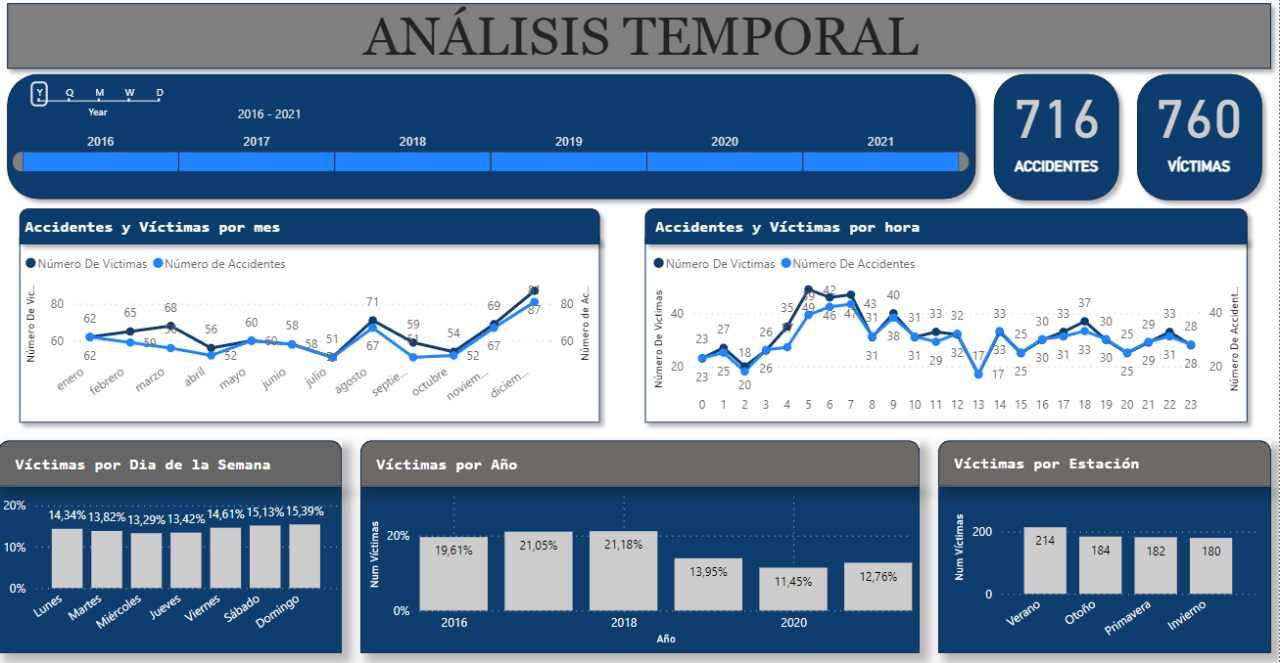
\includegraphics[width=0.8\textwidth]{Tem_Analysis.jpg}
  \caption{Análisis Temporal.}
  \label{fig:tem-analysis}
\end{figure}

\subsection{Análisis Geográfico}
Se realiza también el análisis de la situación geográfica de los accidentes en la ciudad de Buenos Aires, basados en las variables estudiadas, donde se ha encontrado información relevante de la siguiente manera:

\begin{itemize}
    \item La mayor cantidad de accidentes ocurre en avenidas y principalmente en cruces o intersecciones.

    \item Con 98 accidentes que representan el 13,6\% del total de accidentes, la comuna 1 es la comuna con mayor cantidad de accidentes en la ciudad. 

    \item El 51\% de la accidentalidad se encuentra en 5 de las 15 (16 contando los límites) 
    
    \item El barrio Constitución de la comuna 1 registra 36 accidentes, aproximadamente el 37\% de la accidentalidad de la comuna con más accidentes. Esto es porque también es la comuna que más barrios tiene.

    \item La mayor cantidad de accidentes se acumulan hacia el Este de la ciudad.
\end{itemize}

A continuación se presenta un resumen gráfico del análisis hecho. 

\begin{figure}[H]
  \centering
  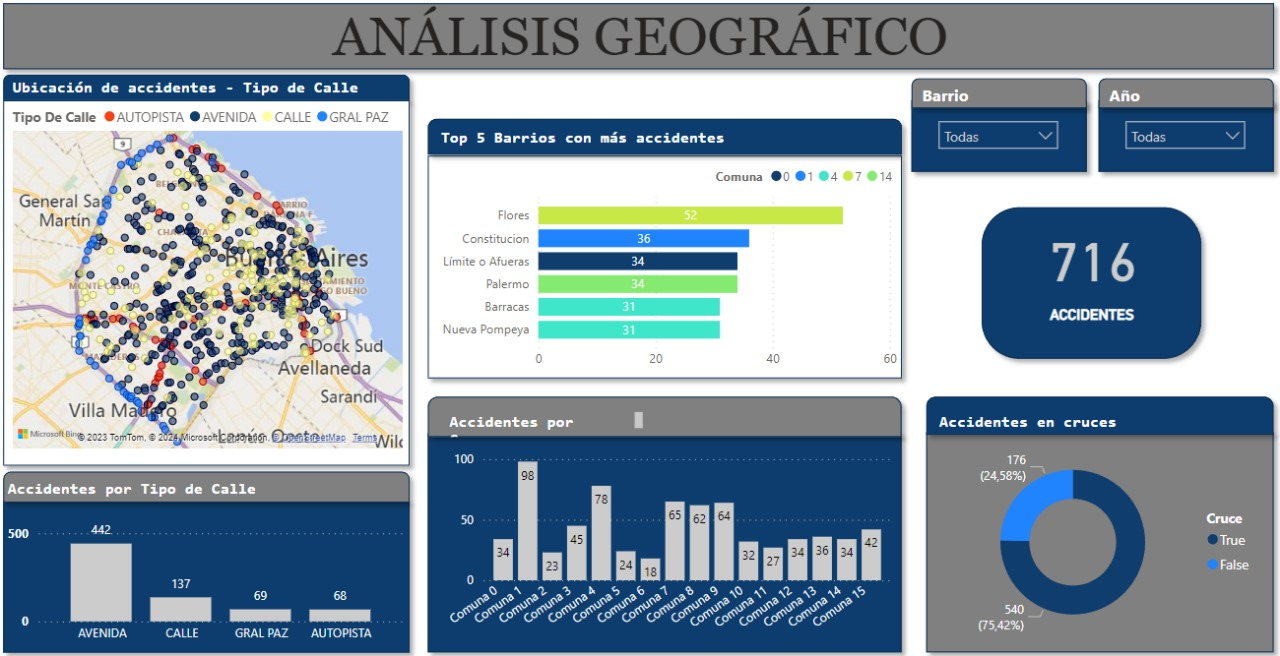
\includegraphics[width=0.8\textwidth]{Geo_Analysis.jpg}
  \caption{Análisis Geográfico.}
  \label{fig:geo-analysis}
\end{figure}

\subsection{Análisis por víctima}
Se realiza también un análisis de víctimas por accidentes de transito en el cual se analizan patrones respecto al rol, la edad, el sexo y el vehículo de los actores involucrados en los accidentes. A partir de este análisis se sacan las siguientes conclusiones:

\begin{itemize}
    \item Los motociclistas y los peatones suman 589 víctimas, equivalente al 77\% total de víctimas.

    \item El número de hombres implicados en un accidente es 3 veces mayor que el número de mujeres. 

    \item La mayor cantidad de hombres accidentados son motociclistas, mientras que la mayor cantidad de mujeres accidentadas son peatonas.
    
    \item El 47\% de las víctimas eran conductores, el 35\% eran peatones y el 18\% restante se distribuye en diferentes roles.

    \item La mayor cantidad de víctimas son adultos entre 26 y 40 años.
    
    \item La mayoría de mujeres víctimas de accidentes viales son adultos mayores de mas de 61 años.

    \item La mayor cantidad de accidentes fueron ocasionados por automóviles.
\end{itemize}

A continuación se presenta un resumen gráfico del análisis hecho. 

\begin{figure}[H]
  \centering
  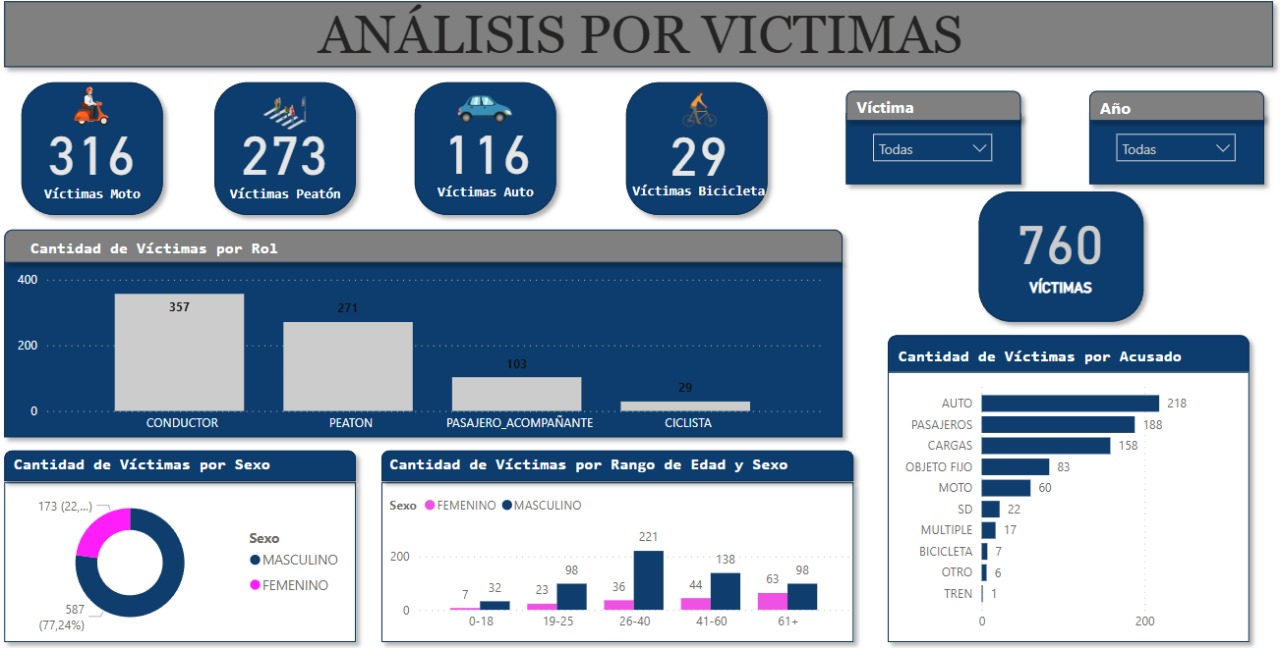
\includegraphics[width=0.8\textwidth]{Vic_Analysis.jpg}
  \caption{Análisis de Víctimas.}
  \label{fig:vic-analysis}
\end{figure}

\subsection{Indicadores Clave de Desempeño (KPI)}
Se plantean 3 indicadores clave de desempeño que permitan evaluar el progreso en la disminución de accidentes y así tomar decisiones efectivas que conlleven a realizar acciones que reduzcan el nivel de accidentalidad en la ciudad de Buenos Aires. A continuación mostraremos los resultados de estos indicadores para el último periodo evaluado, sin embargo las conclusiones finales se tomarán respecto al análisis realizado en conjunto periodo a periodo, sobre la evolución de accidentes. 
\begin{itemize}
    \item \textbf{KPI 1:} Reducir en un 10\% la tasa de homicidios en siniestros viales de los últimos seis meses, en CABA, en comparación con la tasa de homicidios en siniestros viales del semestre anterior.

\begin{figure}[H]
  \centering
  \includegraphics[width=0.8\textwidth]{KPI1.png}
  \caption{KPI 1.}
  \label{fig:KPI 1}
\end{figure}

    Este indicador nos muestra que para el último año el objetivo se cumple, sin embargo no existe una regularidad de cumplimiento relacionada en los años anteriores.
    
    \item \textbf{KPI 2:} Reducir en un 7\% la cantidad de accidentes mortales de motociclistas en el último año, en CABA, respecto al año anterior.

\begin{figure}[H]
  \centering
  \includegraphics[width=0.8\textwidth]{KPI2.png}
  \caption{KPI 2.}
  \label{fig:KPI 2}
\end{figure}

En el último año evaluado el indicador no cumple su objetivo y lo desmejora en un gran porcentaje, aun cuando venía teniendo un comportamiento aceptable en años anteriores, lo cual nos presenta un comportamiento alarmante para este último año 

    \item \textbf{KPI 3:} Reducir en un 5\% la cantidad de accidentes mortales causados por el conductor (Acusado Auto) en el último año

\begin{figure}[H]
  \centering
  \includegraphics[width=0.8\textwidth]{KPI3.png}
  \caption{KPI 3.}
  \label{fig:KPI 3}
\end{figure}

    Este indicador no cumple su objetivo en el último año evaluado y tampoco lo cumple en los años anteriores, razón por la cual se recomienda prestar mayor atención a los accidentes evaluados por este indicador. 
    
\end{itemize}

\section{Conclusiones}
Después de plantear indicadores de desempeño relacionados con el análisis y conclusiones encontradas en cada uno de los tres aspectos evaluados, se encuentra que la reducción de la accidentalidad tiene un comportamiento poco favorable, pues no se cumplen constante ni  certeramente los objetivos en los periodos de tiempo planteados, por lo tanto, se recomienda establecer acciones tales como 
\begin{itemize}
    \item Jornadas de educación vial.
    
    \item Sensibilización a la ciudadanía sobre el impacto social que presenta un siniestro vial.
    
    \item Mayor rigurosidad en las pruebas teóricas y prácticas para la obtención de la licencia de conducir.
    
\end{itemize}
Entre otras, que logren cumplir los objetivos con mayor certeza y regularidad. 
\\
\\
\\
Sin otra particular, quedo atento a sus comentarios, consultas y observaciones.
\\
\\
\\
\section*{Firma}

\\

Leonardo Cortés\\
Analista de Datos \\
Fecha: Enero de 2024


\end{document}